\subsubsection{Software}

Um den Turm zu Steuern musste ein eigenes Softwaremodul entwickelt werden. Dieses sollte Hardware und Datenbank kontrollieren und auf Anfragen Handeln. Ursprünglich war geplant Python als Programmiersprache zu verwenden, da es einfach und simpel ist und man schnell Prototypen entwickeln kann.


\paragraph{V1 - Python}
Die Pythonversion ist basierend auf einem Queue System, bei dem verschiedene Komponenten in verschiedenen \Glspl{thread} selbstständig Jobs und Events hinzufügen können. Ein oder mehrere Job-Handler sollen sich anschließend Jobs aus der Queue entnehmen und ausführen. Ein Job-Handler sollte eine Einlagerungsstation darstellen, somit sollten meherere verschiedene Auslagerungsstationen abgebildet werden können.

\begin{figure}
  \centering
  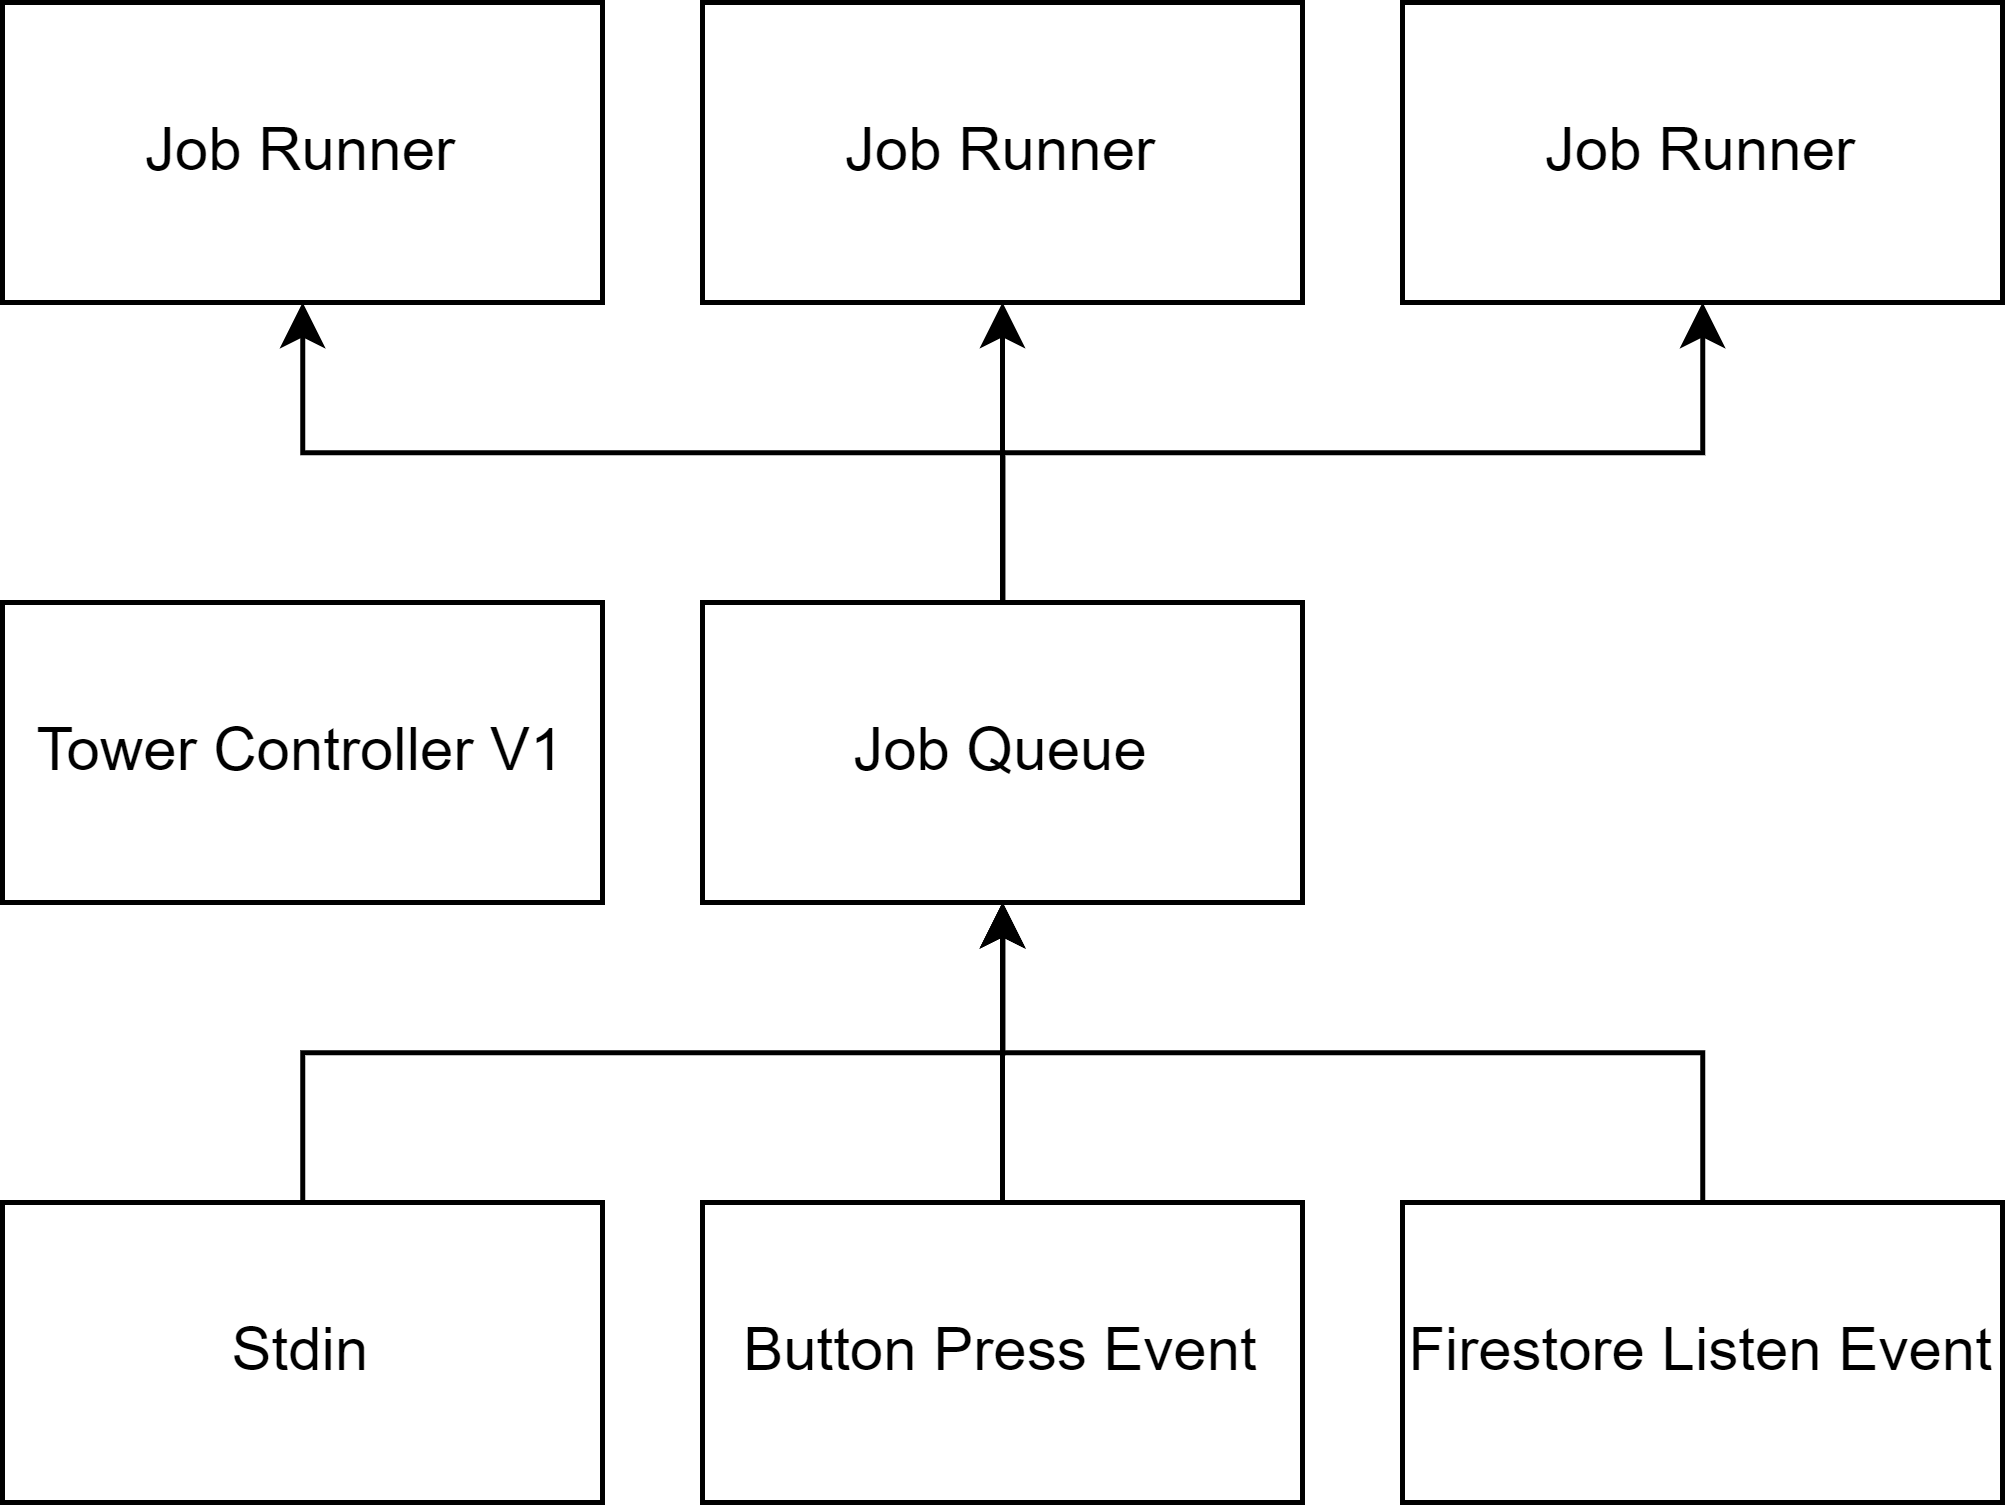
\includegraphics[width=0.5\textwidth]{images/tower_controller_v1.png}
  \caption{Datenströme des Tower Controller V1}
  \label{fig:tower_controller_v1}
\end{figure}

\ac{Stdin} und \ac{Stdout} werden verwendet um mit dem Benutzer zu kommunizieren. \ac{Stdin} wird verwendet, damit ein Benutzer manuell Jobs zur Queue hinzufügen kann. Dies ist vorallem bei zum \Gls{debuggen} nützlich. \ac{Stdout} wird verwendet um dem Benutzer Informationen über den aktuellen Status des Turms zu geben. Eingaben sind eine blockierende Operation, deshalb wurde aioconsole verwendet um \ac{Stdin} asynchron auszuführen.

In einem weiteren \Gls{thread} kommuniziert ein \ac{GPIO} \Gls{listener} mit einem physikalischen Button, welcher zur bestätigung des Einlagerungsvorgangs verwendet werden sollte. Der \Gls{listener} wartet auf einen Tastendruck und fügt anschließend einen Job (\Gls{event}) zur \Gls{queue} hinzu.

Der wichtigste \Gls{listener}ist der Datenbanklistener, dieser wartet auf Änderungen in der Datenbank und fügt entsprechende Jobs zur Queue hinzu. Dieser \Gls{listener} ist essenziell für die Kommunikation zwischen der App und dem Turm. Der \Gls{listener} wird von der offiziellen Python Bibliothek für Firebase bereitgestellt.

Zusätzlich wurde eine \ac{GUI} entwickelt, welche die aktuellen Zustände der einzelnen Radboxen darstellt. Diese \ac{GUI} wird ebenfalls von einem \Gls{thread} ausgeführt und aktualisiert sich automatisch, wenn sich der Zustand der Radboxen ändert. Die \ac{GUI} ist in tkinter implementiert und soll zu bei der Entwicklung helfen, falls das Programm nicht auf dem Raspberri Pi ausgeführt wird oder die Elektrotechnik noch nicht fertig ist.

Die Python Version war zu Anfang vielversprechend, jedoch gab es einige Probleme mit der Architektur, die zu einem komplizierten und unübersichtlichen Code führten. Die Architektur wurde in der V2 komplett überarbeitet.


\paragraph{V2 - Python}
Die Python Version 2 wurde komplett überarbeitet und viel einfacher und übersichtlicher gestaltet. Das Konzept der mehreren Auslagerungsplätze wurde verworfen und es wurde nur ein Auslagerungsplatz implementiert.

Zudem wurde die Architektur komplett überarbeitet. V2 ist basierend auf einer \Gls{statemachine}, die verschiedenen States sind in Abbildung \ref{fig:tower_controller_v1_state_machine} zu sehen.

\begin{figure}
  \centering
  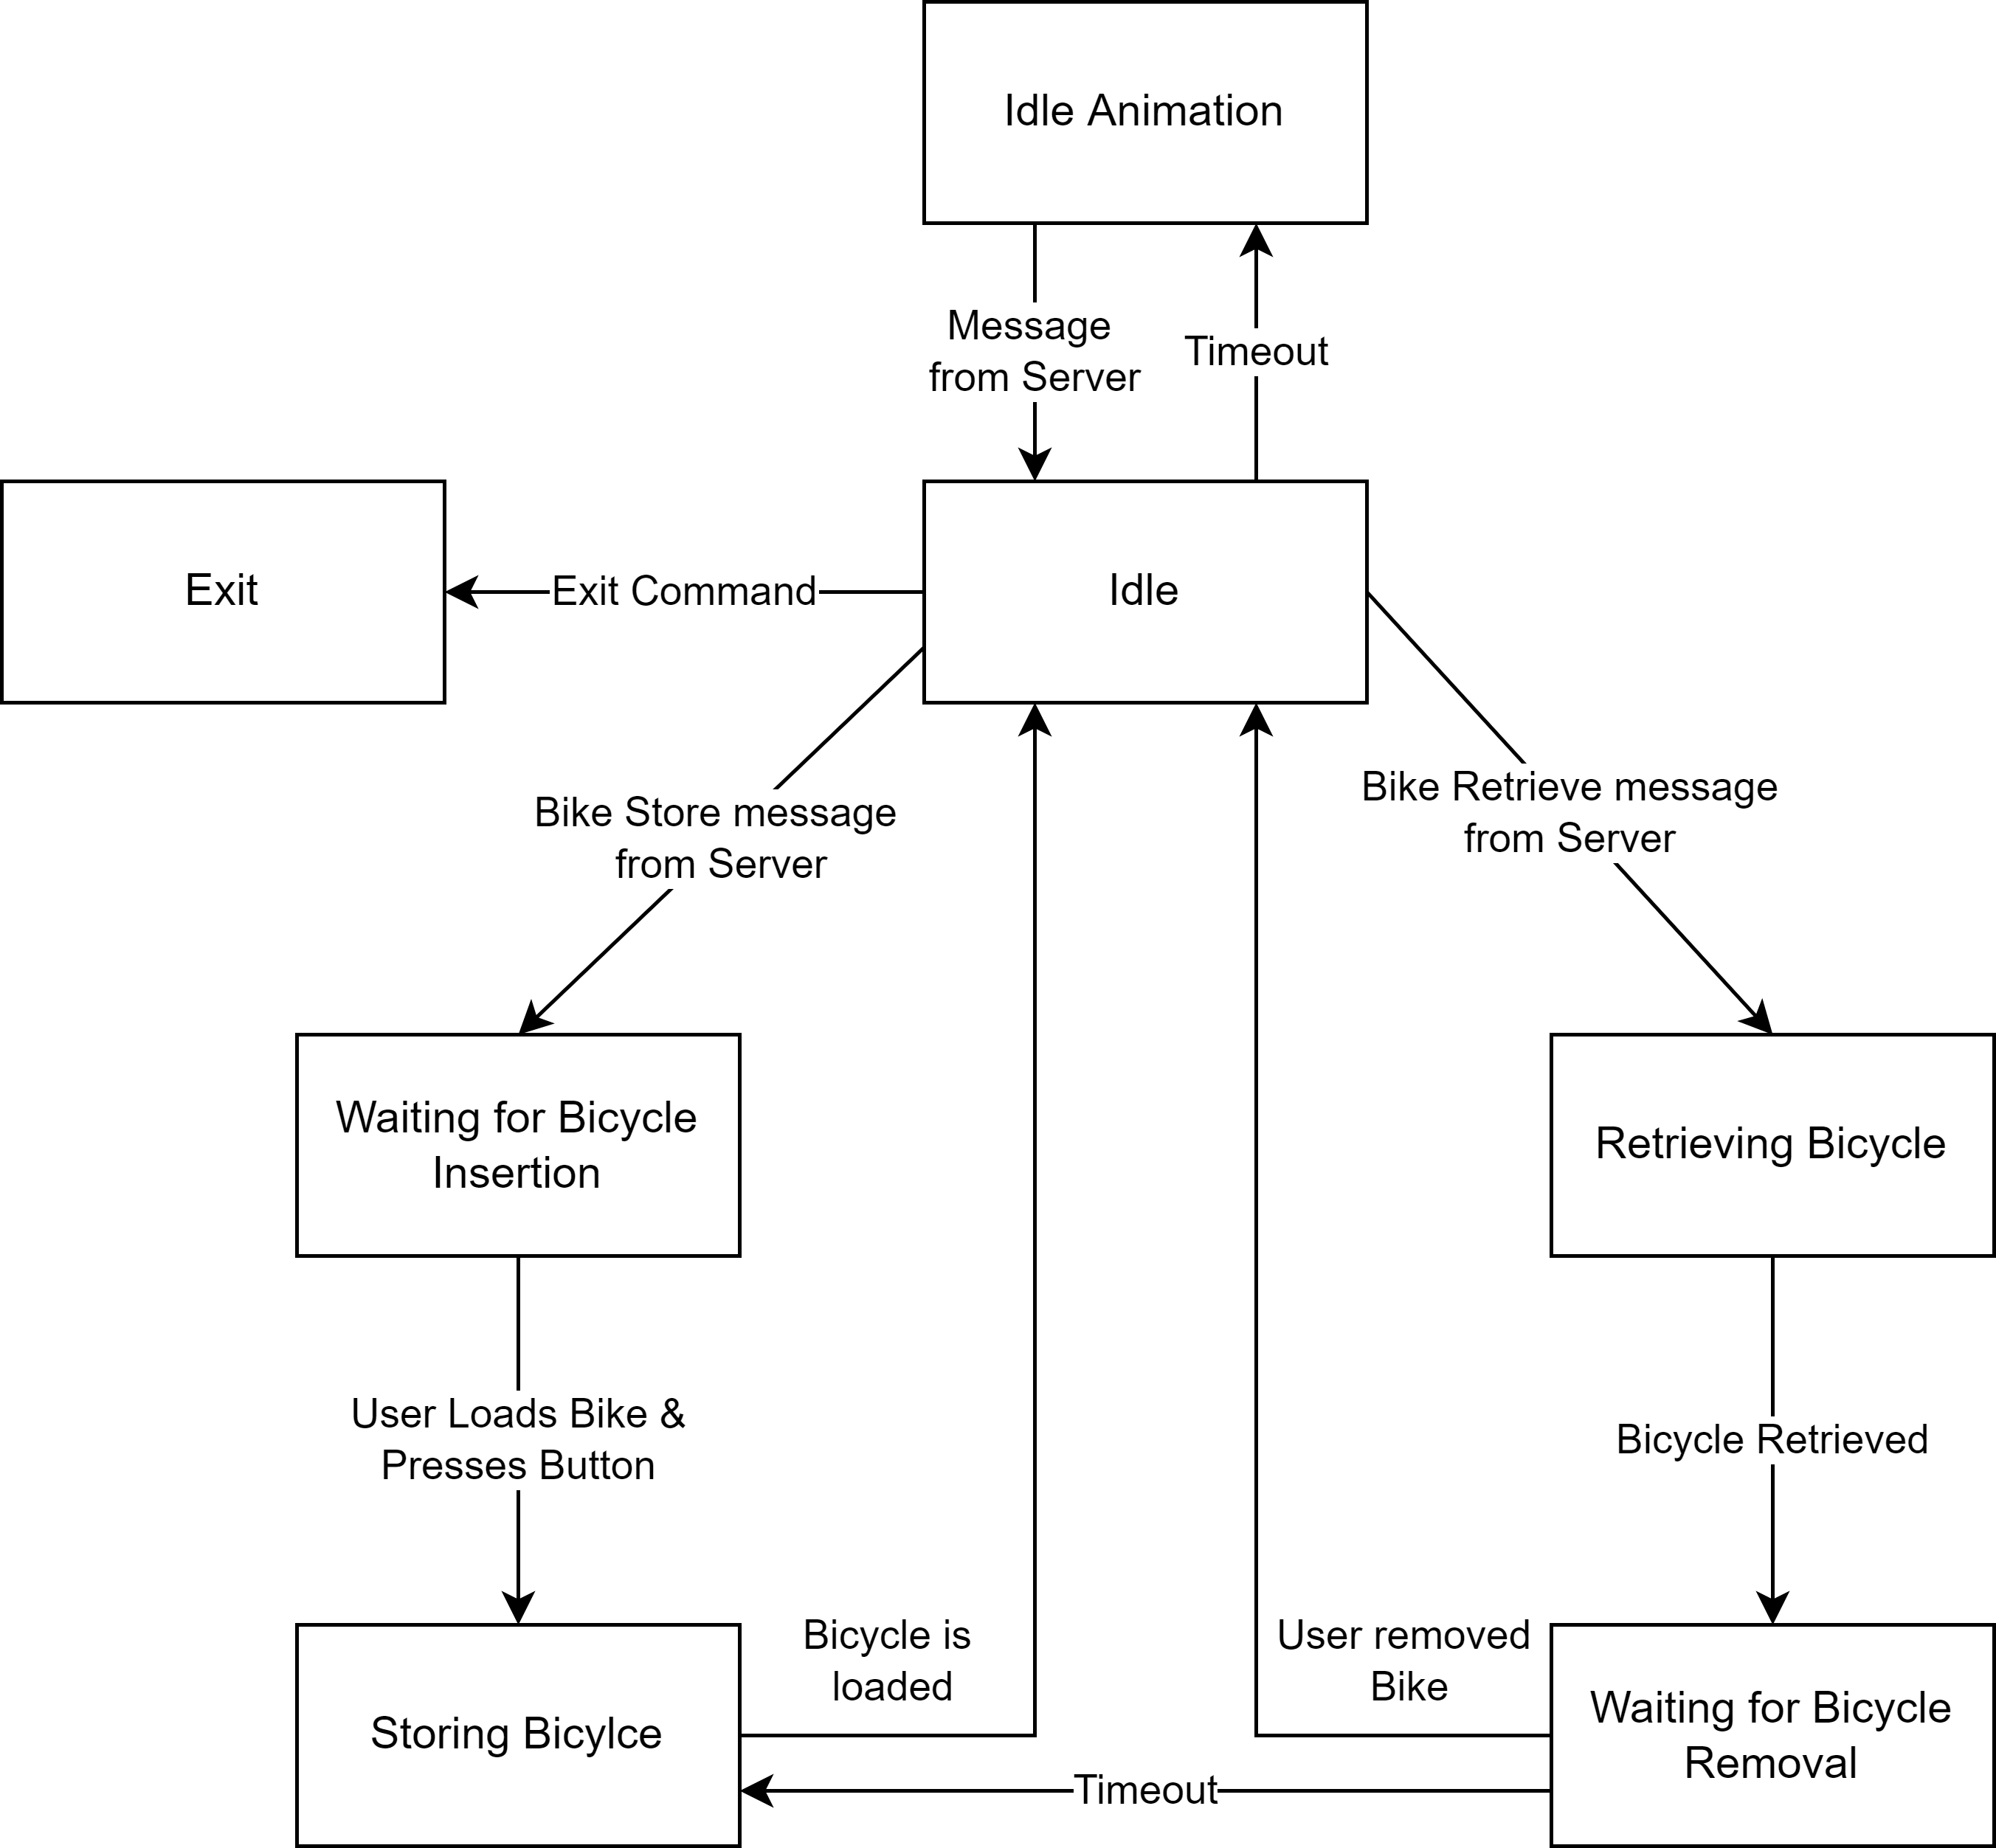
\includegraphics[width=0.8\textwidth]{images/tower_controller_v2_state_machine.png}
  \caption{State Machine des Tower Controller V2}
  \label{fig:tower_controller_v1_state_machine}
\end{figure}

States:
\begin{itemize}
  \item \textbf{Idle} - Der Turm ist im Idle State, wenn er nicht gerade eine Aktion ausführt. In diesem Zustand werden auf \Glspl{event} gewartet. Wenn ein \Gls{event} eintritt, wird der Zustand entsprechend angepasst.
  \item \textbf{Waiting for Bicycle Insertion} - Ein Nutzer hat den Einlagerungsprozess eines Fahrrads gestartet, der Turm wartet nun auf das Einlegen des Fahrrads in die Radbox und die Einlagerungsbestätigung (Drücken des Buttons) des Nutzers.
  \item \textbf{Storing Bicycle} - Das Fahrrad wurde in die Radbox eingelagert und der Nutzer hat die Einlagerungsbestätigung erteilt. Der Turm wartet nun auf das Schließen der Radbox und das Abschließen des Einlagerungsprozesses. Anschließend wird der Zustand wieder auf Idle gesetzt.
  \item \textbf{Retrieving Bicycle} - Ein Nutzer hat den Auslagerungsprozess eines Fahrrads gestartet, der Turm wartet nun auf das Abschließen des Auslagerungsprozesses und das Öffnen der Radbox.
  \item \textbf{Waiting for Bicycle Removal} - Der Turm wartet auf das Entfernen des Fahrrads aus der Radbox und die Auslagerungsbestätigung des Nutzers. Anschließend wird der Zustand wieder auf Idle gesetzt. Falls der Nutzer die Auslagerungsbestätigung innerhalb eines gewissen Zeitraums nicht erteilt, wird der Zustand wieder auf Storing Bicycle gesetzt und das Fahrrad wird eingelagert.
  \item \textbf{Idle Animation} - Falls der Turm für eine gewisse Zeit im Idle Zustand ist, wird eine Animation ausgeführt. Diese Animation soll den Turm visuell ansprechender machen.
  \item \textbf{Exit} - Der Turm Controller wird beendet.
\end{itemize}

Änhlich wie V1 hatte V2 auch eine \ac{GUI}, die den aktuellen Zustand des Turms darstellt. Diese wurde einfach von V1 übernommen und angepasst.

Die V2 Variante funktionierte gut und hätte womöglich auch Architekturell funktioniert, jedoch gab es Probleme mit Python selbst. Die Probleme stammten von zyklischen Importen und erlaubten es nicht die Entwicklung weiterzuführen. Womöglich hätte das Problem gelöst werden können indem auf Type Hints verzichtet worden wäre, jedoch hätte dies die Developer Experience und Lesbarkeit des Codes stark beeinträchtigt. Aus diesem Grund wurde entschieden die Entwicklung von V2 einzustellen und auf eine andere Programmiersprache zu wechseln.


\paragraph{V3 - Rust}
Die V3 Variante wurde in Rust implementiert. Rust ist eine moderne Programmiersprache, die sich durch eine gute Performance und eine gute Developer Experience auszeichnet. Rust unterscheidet sich stark von Python, da es eine Systemsprache ist.

Gegenüberstellung Rust und Python:
\begin{table}[ht]
  \begin{tabular}{l|l|l}
                                      & \textbf{Rust} & \textbf{Python}          \\
    \hline
    \textbf{Typisierung}              & Statisch      & Dynamisch                \\
    \textbf{Garbage Collection}       & Manuell       & Automatisch              \\
    \makecell[l]{\textbf{Performance }                                           \\(100mio Stellen Pi Benchmark\cite{programming_language_speeds})}
                                      & 69.31s        & 5851.53s (84x langsamer) \\
    \textbf{Kompiliert/Interpretiert} & Kompiliert    & Interpretiert            \\
    \textbf{Multi-Thread}             & Ja            & Nein                     \\
  \end{tabular}
  \caption{Gegenüberstellung Rust und Python}
  \label{tab:rust_vs_python}
\end{table}

Rust wurde für V3 gewählt da das zuständige Projektmitglied mehr Erfahrung mit Rust hatte als mit Python. Obwohl Rust komplizierter ist als Python, wurde die Entwicklungsgeschwindigkeit durch die bessere Developer Experience deutlich erhöht.

V3 hatte auch eine \ac{GUI}, die den aktuellen Zustand des Turms darstellt. Diese wurde in \texttt{fltk\_rs} implementiert.

Architekturtechnisch ist V3 sehr ähnlich zu V2. Dennoch stellte sich heraus, dass die Architektur immer noch zu kompliziert war und die Entwicklungsgeschwindigkeit stark beeinträchtigte.


\paragraph{V4 - Rust}

Die V4 Variante wurde ebenfalls in Rust entwickelt, aber von Grund auf neu aufgebaut. Die Architektur wurde komplett überarbeitet und stark vereinfacht. Die \Gls{statemachine} wurde verworfen und die ganze Applikation basiert auf dem Datenbank \Gls{listener}. Der Listener wurde mithilfe Funktionalität der \texttt{firestore\_rs} Softwarebilbiothek Implementiert.

\subparagraph{Projektstruktur}

Das Projekt wurde mit \texttt{cargo new} erstellt, deshalb ist die Projektstruktur wie folgt:

\dirtree{%
  .1 tower\_controller\_v4.
  .2 src.
  .3 bin.
  .3 entities.
}

\begin{itemize}
  \item \textbf{\texttt{tower\_controller\_v4}} Root Verzeichnis des Projekts, hier befinden sich alle    Konfigurationsdateien (Cargo.toml, Cargo.lock, .gitignore, etc\ldots{}).
  \item \textbf{\texttt{src}} Hier befinden sich alle Quellcode Dateien.
  \item \textbf{\texttt{bin}} Hier befinden sich alle Quellcode Dateien, die Ausgeführt werden können.
  \item \textbf{\texttt{entities}} Hier befinden sich die Serialisierbaren Datenstrukturen (Entities), die den Dokumenten in der Datenbank entsprechen.
\end{itemize}

\subparagraph{Programmablauf}
\begin{enumerate}
  \item Der Turm Controller wird mittels der \texttt{main} Funktion gestartet.
  \item Umgebungsvariablen werden geladen.
  \item Datenbank Interface wird erstellt (\texttt{TowerDatabase::new}).
  \item Turm Datenstruktur wird erstellt und mit den Daten aus der Datenbank initialisiert (\texttt{Tower::new}).
  \item Assignment Scheduler wird erstellt (\texttt{AssignmentScheduler::new}).
  \item Der Scheduler wird gestartet (\texttt{AssignmentScheduler::start}) und der main \Gls{thread} wird in einen \Gls{sleep} Modus versetzt.
  \item Das Programm wartet nun auf Änderungen in der Datenbank.
\end{enumerate}

\begin{figure}[ht]
  \centering
  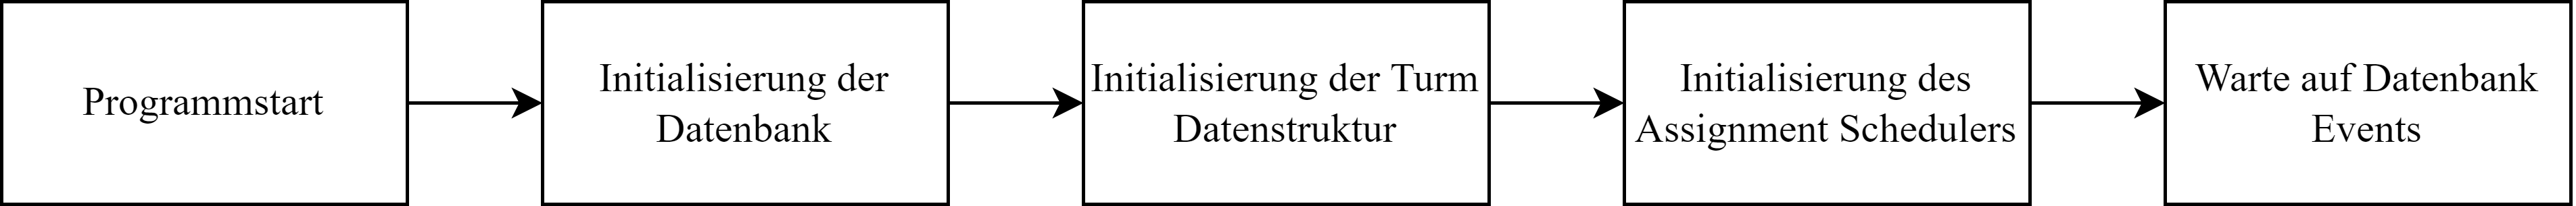
\includegraphics[width=1\textwidth]{images/tower_controller_v4_init.png}
  \caption{Intialisierung des Turm Controllers}
  \label{fig:tower_controller_v4_init}
\end{figure}

\subparagraph{Datenbank Event Handling}

\subparagraph{TowerDatabase}

\subparagraph{Tower}

\subparagraph{AssignmentScheduler}

\subparagraph{TowerDisplay}